\chapter{Progress}
\section{Research}
In the first year of my PhD candidature, I mainly focus on the a SSE scheme that supporting private and efficient boolean query. I and my supervising team design this new SSE scheme named HXT together. The new scheme is based on the `OXT' protocol \cite{cash2013highly}, but its security is further improved by removing a result pattern leakage that leaks the matching pairs of queried keywords. To achieve this, we design a new Hidden Vector Encryption (HVE) scheme without pairing to improve the performance of HVE significantly, and we embedded the new HVE with OXT to hide the result pattern leakage.

A more detailed but concise technical description of our HXT is presented here:

The HXT SSE protocol uses the following primitives (for security parameter $\lambda$):
\begin{itemize}
\setlength{\itemsep}{0pt}
\item A cyclic group $\mathbf{G}$ with prime order $p$ and generator $g$, for which the $\mathbf{DDH}$ assumption holds.
\item A Hidden Vector Encryption scheme $\mathbf{HVE}$.
\item A symmetric key encryption scheme $\mathbf{Sym}$ with key space $1^{\lambda}$.
\item A Bloom filter $\mathbf{BF}$ with length $m$ and $k$ functions.
\item Psuedorandom functions (PRFs) $F$ with range $1^{\lambda}$, $F_p$ with range $\mathbf{Z}^\ast_p$ and  $F_j$ with range $[m]$ for $j=1,\ldots,k$.
\end{itemize}

Likes other SSE schemes, HXT protocol consists of two algorithms: $\mathbf{EDBSetup}$ to create encrypted database and $\mathbf{EDBSearch}$ to query the result from EDB.
 
The setup algorithm $\mathbf{EDBSetup}$ gets the security parameter $\lambda$ and returns $mk$, $param$, and $\mathbf{EDB}$. The encrypted database $\mathbf{EDB}$ has two components: $\mathbf{EDB}(1)$ is $\mathbf{HVE}$  generated exactly as in OXT, and $\mathbf{EDB}(2)$ is an $\mathbf{XSet}$ encryption of a carefully designed Bloom filter $\mathbf{BF}$ set up for $\mathbf{XSet}$ elements of the form $h (\mathbf{id}, w) = g^{F_p (\kappa_X, w ) \cdot \mathbf{xid}}$, for encrypted identifiers $\mathbf{xid}=F_p(\kappa_I,\mathbf{id})$ over all $\mathbf{id}\in\mathbf{DB}(w)$. In particular, this algorithm writes $1$'s into $\mathbf{BF}$ in positions in set 
$$S =\{h_j(\kappa_j,h(\mathbf{id},w))\}_{1\leq j \leq k},$$ 
over all $(\mathbf{id},w)$ pairs with $\mathbf{id}\in\mathbf{DB}(w)$, and then encrypts $\mathbf{BF}$ with $\mathbf{HVE}$.

Similar to OXT, The search protocol generates $\mathbf{stag}$ and $\mathbf{xtoken}$ first. The $\mathbf{XSet}$ membership test for conjunctions in OXT is replaced by a $\mathbf{DB}$ token generation and query. Namely, the $\mathbf{HVE}$ token $\mathbf{token}_c$ is generated for a predicate ($\mathbf{BF}$) vector $\mathbf{v}_c$ with $1$'s in positions in set 
$$S' = \{h_j(\kappa_j,h(\mathbf{id}_c,w_i))\}_{1\leq j\leq k}$$
over all $\mathbf{id}_c \in \mathbf{DB}(w_1)$ and $\mathbf{xterm}$s $w_i$ for $2\leq i\leq n$, and wild-cards in other positions. Consequently (as the message encrypted by $\mathbf{HVE}$ was set to `True' in $\mathbf{EDBSetup}$) the $\mathbf{HVE.Query}$ returns `True' if $S' \subseteq S$, i.e. if \emph{all} $n-1$ $\mathbf{xterm}$s $w_i$ are in the document $\mathbf{id}_c$. Otherwise, $\mathbf{HVE.Query}$ returns $\perp$, without revealing $\mathbf{KPRP}$ information on which $w_i$ are in $\mathbf{id}_c$. Importantly, the $\mathbf{HVE.Query}$ algorithm only uses components of ${\bf c}$ in the non wild-card positions of ${\bf v}_c$ and $\mathbf{token}_c$, so search run-time is only proportional to $|\mathbf{DB}(w_1)| \cdot n \cdot k$ (similar to OXT), and not to the size $m$ of the $\mathbf{BF}$.

Currently the implementation of this scheme in Hadoop is finished and a comparable dataset with OXT is tested in HXT. The result shows that by adopting the in-memory distributed computing framework and distributed database (Spark \cite{apache2017spark} and HBase \cite{apache2017hbase}), the new scheme can perform efficient queries over encrypted database and the overhead of our HVE is almost negligible because it is only use symmetric encryption primitives. 

The paper of HXT is writing in progress, we will test the HXT protocol in a larger dataset as a supplementary result for its efficiency in large scale database. We plan to submit this paper to IEEE S\&P by 1st Dec.

HXT is a more secure SSE protocol that support boolean query functions, and it is also indexed by inverted index. Hence, HXT can serve as a building block of my Searchable Graph Encryption by providing secure and efficient boolean query functions.

\begin{table}[h]
\centering
\begin{tabular}{|c|c|c|}
\hline
\bf Course Code & \bf Course Name & \bf Result \\ \hline
\bf FIT5143 & \bf IT Research Methods & \bf Exempted \\ \hline
\bf  FIT6021 & \bf Advanced Research Methods & \bf C \\ \hline
& Argument Analysis & HD \\ \hline
& Problem Solving and Proof & D \\ \hline
& Scientific Method & HD \\ \hline
& Modelling and Computer Simulation & Attended but Missing \\ \hline
& Design Research & D \\ \hline
\bf FIT5144 & \bf MGE Monash Graduate Research & \bf 4 hours \\ 
& \bf Student Induction &  \\ \hline
\bf FIT5144 & \bf MGE  Research Integrity & \bf 12 hours \\ \hline
\bf FIT5144 & \bf Faculty of IT Induction & \bf 6 hours \\ \hline
\bf FIT5144 & \bf Communicating Research & \bf 30 hours\\ \hline
& Strategies and Plans & completed \\ \hline
& Academic Audiences & completed \\ \hline
& Funding Applications & completed \\ \hline
& Community Audiences & completed \\ \hline
& Lay Audiences & completed \\ \hline
\bf FIT5144 & \bf Ethical Research and Publications & \bf 6 hours\\ \hline
& Philosophical Approaches of Ethic & completed \\ \hline
& Ethic in Publication and Authorship & completed \\ \hline
\end{tabular}
\caption{Coursework Activities and Claimed Hours}
\label{tlb:coursework}
\end{table}

\section{Courseworks}
To meet the coursework requirements, I've get exemption for one compulsory module and attend another one as well as the compulsory events and workshops in FIT 5144 in the first year. However, there are some issues with my grades in FIT6021 module ``Modelling and Computer Simulation''. Table \ref{tlb:coursework} shows the detailed information about my coursework activities. 

Apart from the compulsory 58 hours' events and workshops listed above, I also attend GSAS Oral Presentations Workshops, Preparing for Confirmation Workshops; The Data61 reading group; Dean's Seminar Series; Staff Appointment Seminar in FIT as elective activities to fulfil the requirement of 120 hours activities attending record for FIT5144.


\chapter{Timeline to Completion}
\begin{figure}[h]
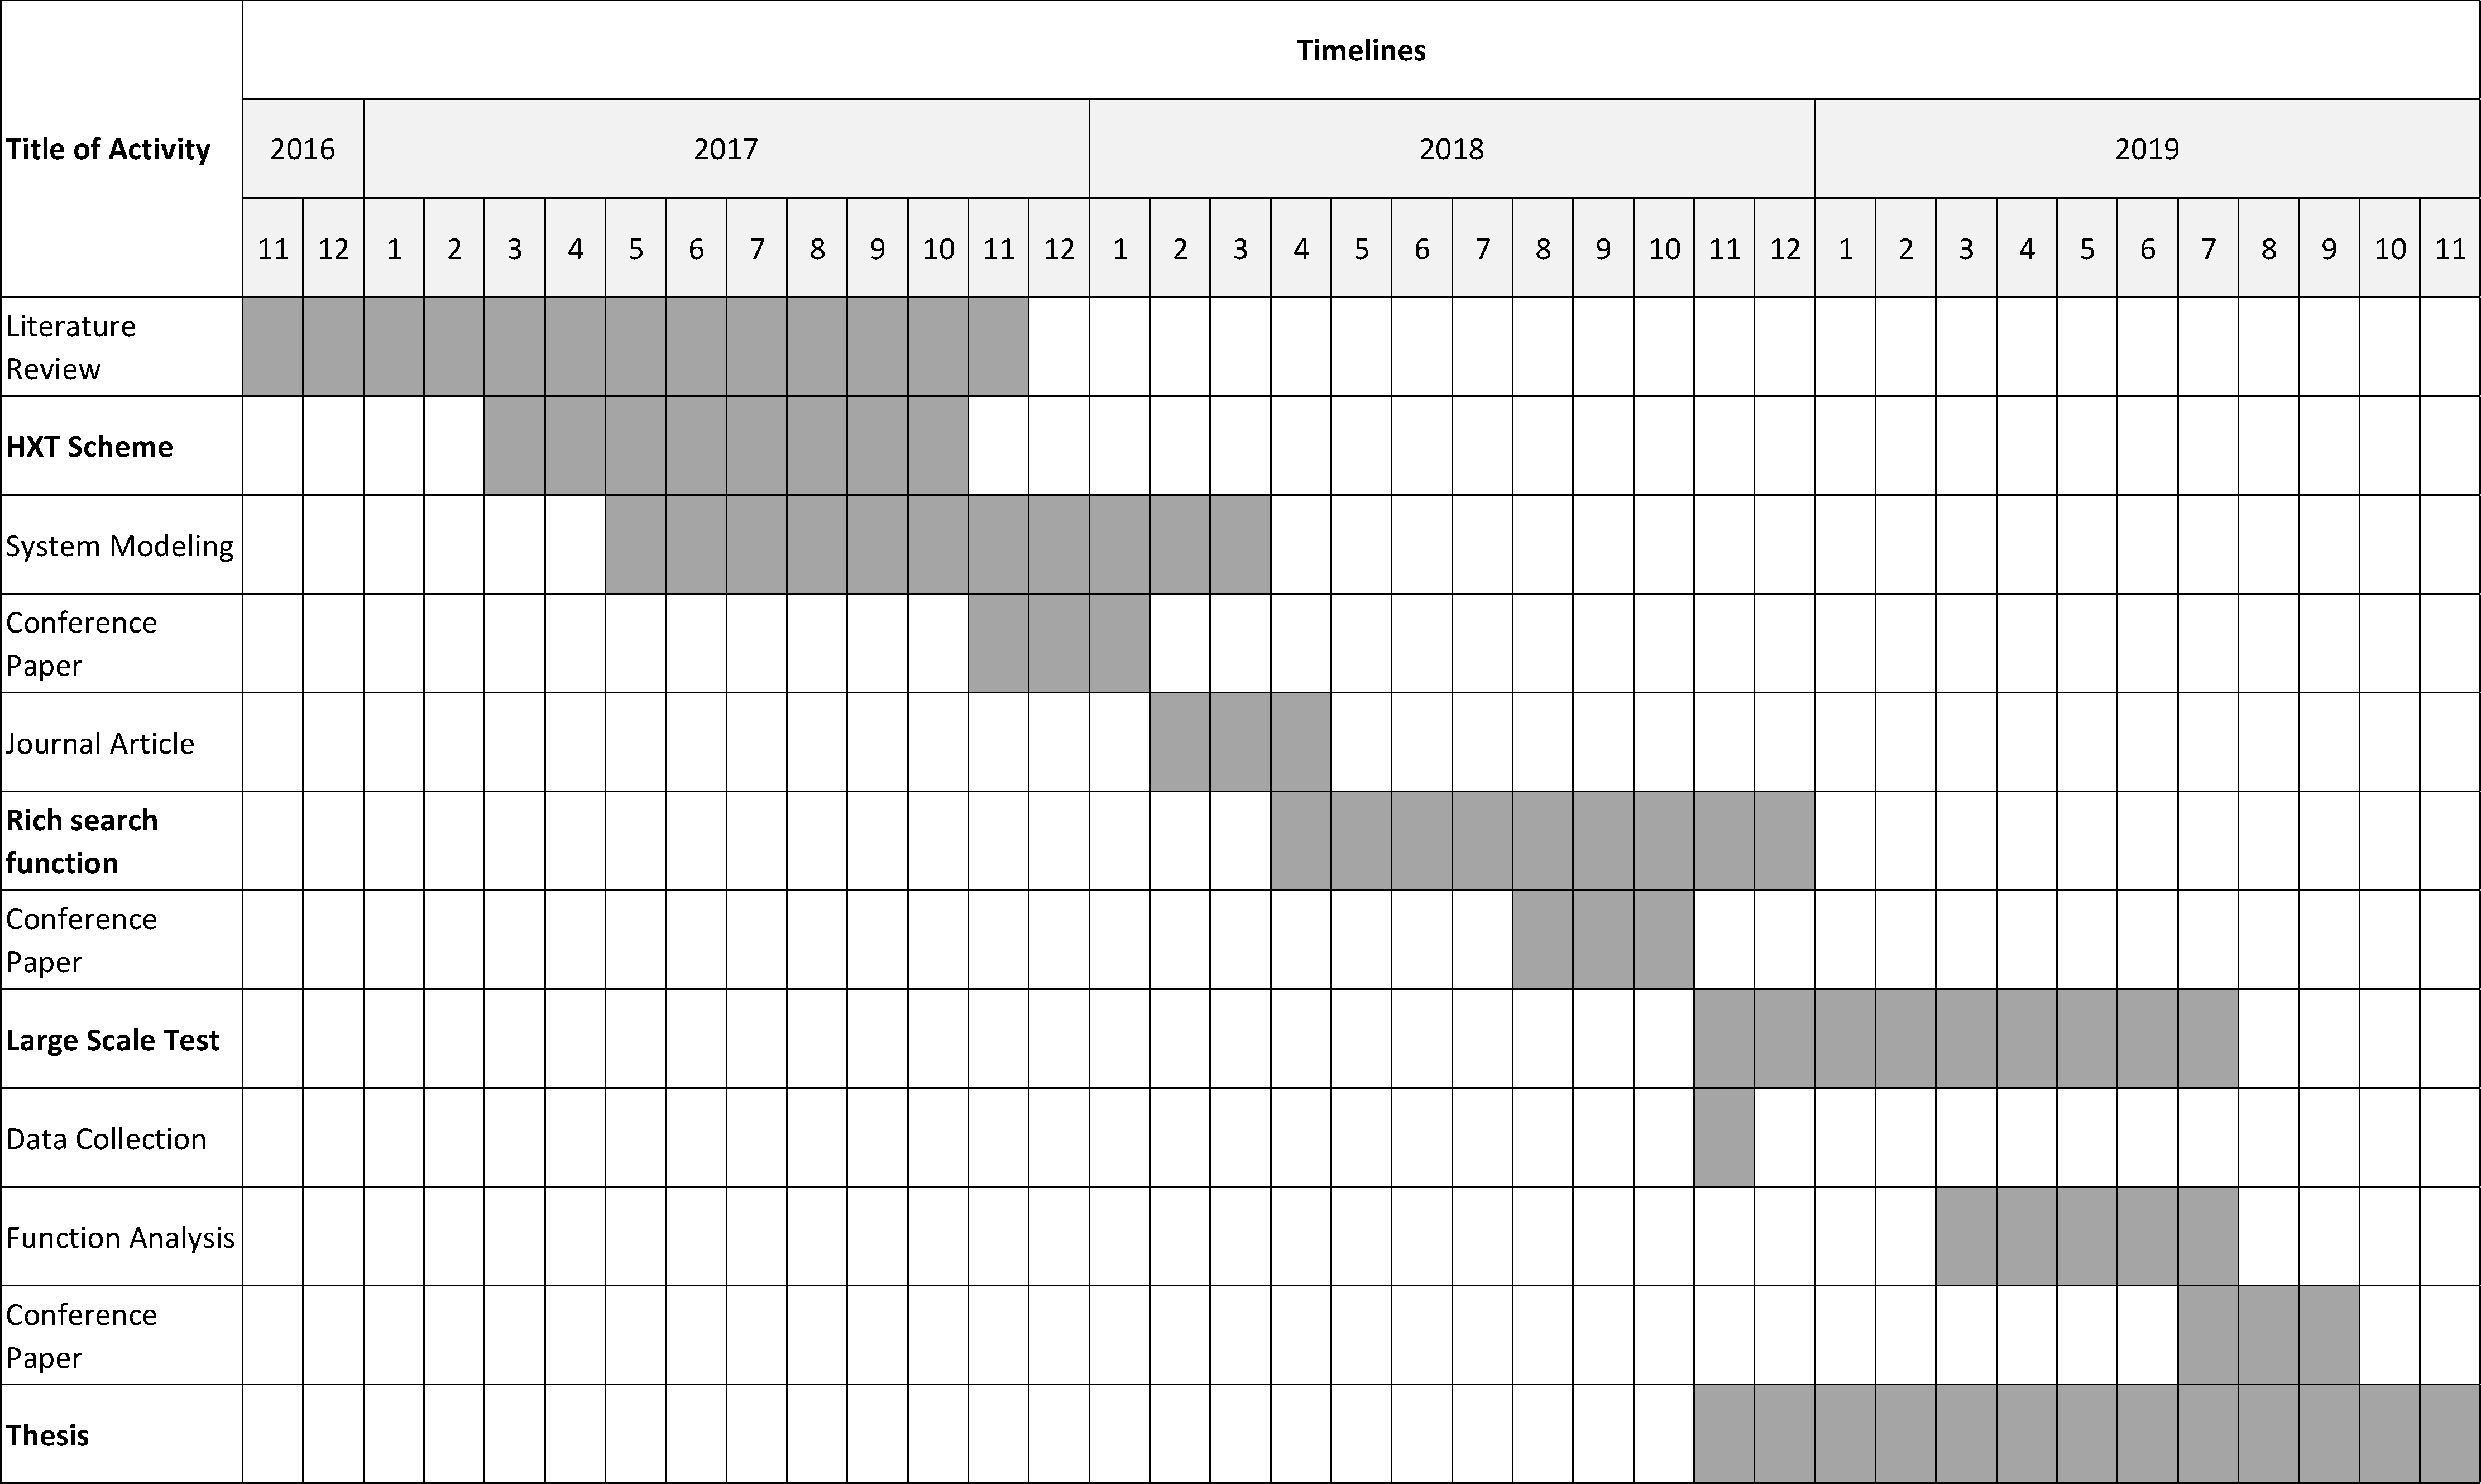
\includegraphics[width=\textwidth]{timeline.pdf}
\end{figure}
